\newpage
% \section{宇宙大尺度结构}
% 书 P2

\section{宇宙学基本框架}
\subsection{宇宙学原理}
现代宇宙学的一个基本假设就是宇宙学原理: 宇宙是均匀且各向同性的. 也可以表述为: 宇宙不同地点, 同一时刻看到的宇宙图像是一样的, 其演化也是一样的. 
\begin{figure}[!htb]
    \centering
    \begin{minipage}{0.24\textwidth}
        \centering
        \begin{tikzpicture}
            \draw [<->, thick] (3,0)--(0,0) node [below left] {$O$}--(0,3);

            \draw [->] (0, 0)--(45:2);
            \draw [->] (0, 0)--($(45:2)+(0, 0.8)$);
            \node at (22:0.5) {$\theta$};

            \draw [dashed] (45:2)--($(45:2)+(0, 0.8)$) node [midway, right] {$ds$};
        \end{tikzpicture}
        \caption{二维平面}
    \end{minipage}
    \begin{minipage}{0.24\textwidth}
        \centering
        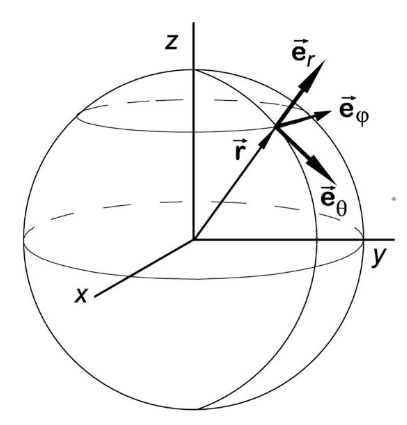
\includegraphics[width=\textwidth]{GA8/二维球面}
        \caption{二维球面}
    \end{minipage}
\end{figure}

研究宇宙的第一步是刻画一个时空的几何结构. 考虑一个均匀各向同性的2维平面
\begin{align*}
    d^2 s=d^2 r+r^2d^2\theta
\end{align*}

考虑一个二维球面, 其线元为
\begin{align*}
    d^2 s&=r^2d^2\theta+r^2\sin^2\theta d^2\varphi\\
    &=r^2 (d^2\theta+\sin^2\theta d^2 \varphi)
\end{align*}

为将这2者写为统一的形式, 令 $x=\sin\theta,\ dx=\cos\theta d\theta$
\begin{align*}
    d^2 s=r^2 \left( \frac{d^2 x}{1-x^2}+x^2d^2\varphi \right)
\end{align*}
引入空间曲率因子$K$, 对于平面$K=0$, 对于球面, $K=1$, 则二维平面的线元可以写为
\begin{align*}
    d^2 s=a^2(t) \left( \frac{d^2 x}{1-Kx^2}+x^2d^2\varphi \right)\ \left\{\begin{array}{ll}
        K=0 & \text{平面} \\
        K=1 & \text{球面} \\
        K=-1& \text{双曲面} 
    \end{array} \right.
\end{align*}
这里$a(t)$是空间尺度因子, 可以是时间的函数. 

对于一个均匀各向同性的三维空间, 可以将其想象成为四维空间中的球面. 与三维空间中推导2D球面类似, 三维球面的线元之间的距离可以写成
\begin{align}
    d l^2=a^2(t)\left[ \frac{d r^2}{1-K r^2}+r^2(d \vartheta^2 +\sin^2 \vartheta d \psi^2 ) \right] \label{E0}
\end{align}
它类似于球坐标下距离的表达式. $(r, \vartheta, \varphi)$是共动坐标, 是不随着尺度因子而变化的(可以想象为下图膨胀球面上的坐标).  $r$是无量纲的, 转换为物理距离$(x)$时需要乘以尺度因子$a$. 

\begin{figure}[!htb]
    \centering
    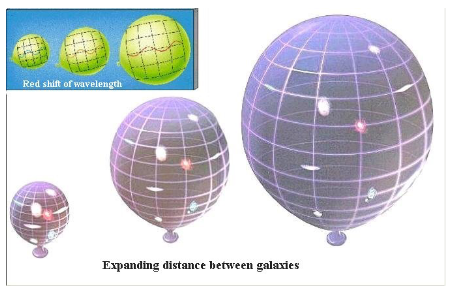
\includegraphics[width=0.309\textwidth]{GA8/四维球面}
    \caption{四维球面}
\end{figure}

对于两个分别处在 $(r=0, \vartheta, \varphi)$, $(r, \vartheta, \varphi)$ 的星系, 其物理距离 $D$ 可表示为
\begin{align*}
    D&=a(t)\int \frac{dr}{\sqrt{1-Kr^2}}=a(t)*\chi (r)\\
    \chi (r) &=\left\{ \begin{array}{ll}
        \arcsin r & K=1\\
        r & K=0\\
        \ln(r+\sqrt{r^2+1}) & K=-1
    \end{array} \right.
\end{align*}

两个星系之间的相对物理速度
\begin{align*}
    v&=\frac{d D}{dt}+\frac{d(a \chi(r))}{dt} \\
    &=\frac{\dot{a}}{a}D+\dot{\chi}a
\end{align*}
$\frac{\dot{a}}{a}D$为空间膨胀引起的速度, $\dot{\chi}a$为星系位置变化引起的速度 (共动坐标), 大部分情况下$\frac{\dot{a}}{a}D>\dot{\chi}a$. (超光速是相对速度不可超光速, 但算上膨胀速度可能超过光速)

定义哈勃常数
\begin{align*}
    H=\frac{\dot{a}}{a}
\end{align*}
因此有$v=HD$. 

哈勃常数不依赖于空间位置, 只是个时间的函数. 取宇宙当前时刻$t=t_0$, 则$H=H_0$, $H_0$表示目前测量的哈勃常数. 这就是熟悉的哈勃定律, 即星系的相对速度与距离成正比. 

\begin{enumerate}\small
    \item 从 $v=HD$可以看到, 哈勃常数的单位为km/s/Mpc. 
    \item 目前测量的哈勃常数$H_0 \cong  67$-73km/s/Mpc, 即在1Mpc的距离上, 星系的相对速度$\sim$70km/s
    \item $1/H=D/V$, 为时间的量纲, 即星系用100hkm/s的速度分开到1Mpc需要的时间, 大致为宇宙年龄. $t\sim 1/H_0 =9.78*10^9 $hyr, 代入$h\sim 0.7, t\sim 139$亿年
\end{enumerate}

考虑时间作为第四维, 则空时间隔为
\begin{align}
    ds^2=c^2 dt^2-a^2(t)\left[ \frac{dr^2}{1-Kr^2}+r^2(d\vartheta^2 + \sin^2\vartheta d \varphi^2) \right] \label{E1}
\end{align}
这就是著名的Robertson-Walker度规. 他们分别独立证明了上式是满足均匀和各向同性要求的唯一四维时空. 该度规也称为Friedmann-Robertson-Walker metric (FRW), 或者FLRW度规与狭义相对论类似, 
\begin{itemize}\small
    \item 称$ds>0$为类时间隔
    \item 称$ds<0$为类空间隔
    \item 称$ds=0$为光子测地线
\end{itemize}

\subsection{宇宙学红移(cosmic redshift)}
几乎所有天文观测都是通过接受天体的辐射, 因此需要了解光子在FRW中的传播过程对于光子, 其沿着测地线传播, 即$ds=0$. 将光子看出波, 考虑一个波峰沿径向传播$(d\vartheta= d\varphi=0)$,其在$t_e$时刻从距离$r$处发出, 到今天被观测者接收到$(r=0, t_0)$由上述等式得到
\begin{align*}
    \int_{t_e}^{t_0}\frac{dt}{a(t)}=\int_0^r\frac{dr}{\sqrt{1-Kr^2}}
\end{align*}
其下一波峰在$t_e+\Delta t_e$时刻发出, 在$t_0 + \Delta t_0$时刻被接受到, 则有
\begin{align*}
    \int_{t_e+\Delta t_e}^{t_0+\Delta t_0}\frac{dt}{a(t)}=\int_0^r\frac{dr}{\sqrt{1-Kr^2}}
\end{align*}
由于光源和接受者的共动位置没有变化, 即满足
\begin{align*}
    \int_{t_e}^{t_0}\frac{dt}{a(t)}=\int_{t_e+\Delta t_e}^{t_0+\Delta t_0}\frac{dt}{a(t)}
\end{align*}
将右边展开为
\begin{align*}
    \int_{t_e+\Delta t_e}^{t_0+\Delta t_0}\frac{dt}{a(t)}=\int_{t_e+\Delta t_e}^{t_e}\frac{dt}{a(t)}+\int_{t_e}^{t_0}\frac{dt}{a(t)}+\int_{t_0}^{t_0+\Delta t_0}\frac{dt}{a(t)}
\end{align*}
可以得到
\begin{align*}
    &\int_{t_e+\Delta t_e}^{t_e}\frac{dt}{a(t)}+\int_{t_0}^{t_0+\Delta t_0}\frac{dt}{a(t)}=0\\
    &\int_{t_e}^{t_e+\Delta t_e}\frac{dt}{a(t)}=\int_{t_0}^{t_0+\Delta t_0}\frac{dt}{a(t)}
\end{align*}
当$\Delta t_e$与$\Delta t_0$都很小时, 可得
\begin{align*}
    \frac{\Delta t_0}{a(t_0)}=\frac{\Delta t_e}{a(t_e)}
\end{align*}
由于光子的波长正比于其波峰之间的时间间隔, 因此接收到的波长$\lambda_0$ 与发出波长$\lambda_e$ 之比为
\begin{align*}
    \frac{\lambda_0}{\lambda_e}=\frac{\Delta t_0}{\Delta t_e}=\frac{a(t_0)}{a(t_e)}
\end{align*}
波长的变化完全由宇宙的膨胀因子$a(t)$决定. 

定义红移$z$(redshift)
\begin{align}
    z=\frac{\lambda_0-\lambda_e}{\lambda_e}=\frac{a(t_0)}{a(t_e)}-1 \label{E2}
\end{align}
这就是宇宙学红移. (目前最重要的公式之一)

由于宇宙膨胀, 令$a(t_0)=1$, 则 $a(t)<1, z>0, (t<t_0)$:
\begin{itemize}\small
    \item 对于本地宇宙 $z=0$
    \item 对于极早期宇宙 $a\sim 0, z\sim \infty$
    \item 对于宇宙微波背景辐射 $z\sim 1000$
\end{itemize}

\subsection{星系的红移}
不同红移的概念. 
\begin{itemize}\small
    \item 多普勒红移, $z_d=\frac{v}{c}$
    \item 宇宙学红移 $z_c=\frac{a(t_0)}{a(t_e)}-1$
\end{itemize}
他们的来源完全不一样. 一个是由于物体相对于观测者运动引起, 另一个是由宇宙膨胀引起. 但是当红移$z\ll 1$时, 宇宙膨胀引起的红移与多普勒红移是等价的. 

一般来说, 观测的星系红移时其多普勒红移与哈勃红移的叠加. 

对于星系, 在其发出光子处, 由于多普勒效应, 其波长相对本地实验室变化为 
\begin{align*}
    \lambda_e'=(1+z_d)\lambda_e
\end{align*}
由于宇宙学红移, 今天的观测者测量的波长
\begin{align*}
    \lambda_0=(1+z_c)\lambda_e'=(1+z_c)(1+z_d)\lambda_e
\end{align*}
因此, 观测到的红移
\begin{align*}
    1+z_0&=(1+z_c)(1+z_d)\\
    z_0&=z_c+z_d +z_c z_d
\end{align*}
实际上我们只能测量$z_0$, 并不能测量$z_c$. 但是由于多普勒效应导致的红移$z_d<0.01$, 因此对于$z_c>0.05$, 一般来说都是宇宙学红移占主导. 

\subsection{Firedmann 方程}
给定宇宙的几何度规, 即RW度规以后, 宇宙的演化(尺度因子$a(t)$由爱因斯坦场方程决定)
\begin{align}
    R_{\mu\nu}-\frac{1}{2}g_{\mu\nu}R-g_{\mu\nu}\Lambda=\frac{8\pi G}{c^4}T_{\mu\nu}\label{E3}
\end{align}
$R_{\mu\nu}$为 Ricci 张量, $R$为曲率标量, $g_{\mu\nu}$ 为空间度规, $T_{\mu\nu}$ 为能量动量, $\Lambda$为宇宙学常数. (完全理解\ref{E3}的意义, 需要广义相对论基础知识, 不是本课程的重点)

对于均匀各性同性宇宙, 可以用理想流体,密度为$\rho$, 压强为$P$, 来描述宇宙物质的能量动量张量, 且流体只有时间分量. 在一系列简化假设之后, 有爱因斯坦场方程的时-时分量
\begin{align}
    \frac{\ddot{a}}{a}=-\frac{4\pi G}{3}\left( \rho+3\frac{P}{c^2} \right)+\frac{\Lambda c^2}{3} \label{E4}
\end{align}
与场方程的空间-空间分量
\begin{align}
    \frac{\ddot{a}}{a}+2\frac{\dot{a}^2}{a^2}+2\frac{Kc^2}{a^2}=4\pi G\left( \rho-\frac{P}{c^2} \right) +\Lambda c^2\label{E5}
\end{align}
根据\ref{E4}与\ref{E5},可得到
\begin{align}
    \left( \frac{\dot{a}}{a} \right) ^2=\frac{8\pi G}{3}\rho -\frac{K c^2}{a^2} +\frac{\Lambda c^2}{3}\label{E6}
\end{align}
\ref{E4}与\ref{E6}, 被称为Friedmann方程. 

Friedmann方程给出2个方程, 但有三个未知数, $a(t)$, $\rho(t)$, $P(t)$. 因此, 要得到宇宙膨胀因子$a(t)$, 必须还要知道状态方程, 即$P$与 $\rho$的关系, 或者他们与膨胀因子$a$的关系. 

特殊情况: 爱因斯坦宇宙模型. 根据Freidmann方程\ref{E6}, \ref{E4}, 可以看到, 在没有宇宙学常数, 即$\Lambda=0$, 且在物质压强$P=0$的情况下, 宇宙不能保持静止状态, $\ddot{a}\ne 0$. 当时爱因斯坦, 包括几乎所有人, 都认为宇宙应该处于静止状态. 因此爱因斯坦给他的场方程添加了宇宙学常数$\Lambda$. 
\begin{itemize}\small
    \item 若 \ref{E4}$=0$, 可得$\rho=\frac{\Lambda c^2}{4\pi G}$, 且很显然$\rho > 0, \Lambda>0$
    \item 若 \ref{E6}$=0$, 由$K=[-1,0,1]$, 可得$K=1$, 且$a=\frac{1}{\sqrt{\Lambda}}$
\end{itemize}
即宇宙的物质密度$\rho$, 尺度因子$a$分别满足上述要求时, 宇宙可以保持静止状态实际上, 即使满足上述条件, 宇宙也是处于不稳定状态, 如果一个微扰, 导致: 
\begin{itemize}\small
    \item $\dot{a}>0$ , 宇宙塌缩, 则密度$\rho \uparrow$, 导致 $\ddot{a}<0$, 宇宙继续塌缩
    \item $\dot{a}>0$ , 宇宙膨胀, 则密度$\rho \downarrow$, 导致 $\ddot{a}>0$, 宇宙继续膨胀
\end{itemize}

\subsubsection{热力学和状态方程}
为了求解Friedmann方程, 必须知道物质的密度$\rho$和压强$P$随着时间的变化, 或者随着宇宙膨胀因子$a$的变化.

考虑某一体积$V(\sim a(t)^3)$内理想流体的热力学过程. 根据热力学第一定律, 系统的内能变化为, $dU=dQ+dW$, $dQ$为系统与外界的热量交换, $dW$为做功. 由于宇宙均匀, 因此系统与外界没有热量交换$(dS=\frac{dQ}{T}=0)$, 因此对于绝热过程, $dU+PdV=0$, $P$为压强. 单位体积的内能$\varepsilon=\rho c^2$, 宇宙的能量密度来源于普通物质, 辐射, 真空能, 即
\begin{align*}
    \rho c^2=\rho_m c^2+\rho_m K+\frac{4\sigma_{SB}}{c}T^4+\rho_{vac}c^2
\end{align*}
这里$\rho_m$为物质密度, $K$为其热能$\left(\frac{3}{2}kT\right)$, $\frac{4\sigma_{SB}}{c}T^4$ 为辐射能量密度,  $\rho_{vac}c^2$ 为真空能量密度. 

由$dU+PdV=0$, 可得
\begin{align*}
    d(\rho c^2 V)+Pd V&=0\\
    Vd \rho + \left(\rho +\frac{P}{c^2}\right)d V&=0
\end{align*}
由于$V\sim a^3$, $dV\sim 3a^2da$可得
\begin{align*}
    \frac{d\rho}{da}+3\left( \frac{\rho+\frac{P}{c^2}}{a} \right)=0
\end{align*}
一般定义物质的状态方程为$P=w\rho c^2$, 代入上式可得
\begin{align*}
    \rho \propto a^{-3(1+w)}
\end{align*}

对于以下三种极端情况, 可以得到密度随膨胀因子$a$的演化:
\begin{enumerate}\small
    \item 冷物质 (非相对论性物质 (普通物质, 暗物质), 压强相对于物质内能很小): $P=0, w=0, \rho \propto a^{-3}$
    \item 热物质 (相对论性物质, 如辐射): $P=\frac{\rho}{3}, w=\frac{1}{3}, \rho\propto a^{-4}$. 由于 $\rho\propto \frac{4\sigma_{SB}}{c}T^4$, 可得 $T\propto a^{-1}$, 即辐射的温度随着膨胀因子反比变化. 
    \item 真空能 (与$a$无关): 即$w=-1, P=-\rho c^2$, 因此真空能为负压
\end{enumerate}

从观测可知: 
\begin{enumerate}\small
    \item 对于目前宇宙, 其物质(主要
    为非相对论性暗物质)密度$\sim 10^{-29}$g/cm${}^3$, 辐射(宇宙微波背景)的密度$\sim 10^{-33}$g/cm${}^3$, 目前宇宙为物质主导
    \item $z\sim 1000(a\sim 10^{-3})$ 物质主导
    \item $z\sim 10000$ 物质与辐射密度大致相当
    \item $z>10000$ 辐射主导
\end{enumerate}

\subsubsection{Firedmann 方程求解}
\begin{align*}
    \left( \frac{\dot{a}}{a} \right)^2&= \frac{8\pi G}{3}\rho-\frac{Kc^2}{a^2}+\frac{\Lambda c^2}{3}
\end{align*}
利用上述关于物质密度随膨胀因子a的变化, 并定义暗能量密度 $\rho_{\Lambda}=\frac{\Lambda c^2}{8\pi G}$, 可得
\begin{align}
    \left( \frac{\dot{a}}{a} \right)^2
    =\frac{8\pi G}{3}\left[ \rho_{m,0}\left( \frac{a_0}{a} \right)^3+\rho_{r,0}\left( \frac{a_0}{a} \right)^4 +\rho_{\Lambda} \right]-\frac{K c^2}{a^2} \label{E7}
\end{align}
不用求解\ref{E7}, 我们可以大致得到宇宙膨胀因子$a$随时间的变化[\ref{T1}]. 

\begin{table*}[!htb]
    \centering
    \caption{宇宙膨胀因子$a$随时间的变化}
    \label{T1}
    \begin{tabular}[c]{cccc}\toprule
        & $K=-1$ & $K=0$ & $K=1$ \\ \midrule
        $\Lambda>0$ & $\dot{a}>0$ 未来一直膨胀 & $\dot{a}>0$ 未来一直膨胀 & \begin{tabular}[c]{@{}l@{}}
            $\rho_{m,0}+\rho_{r,0}\gg \rho_\Lambda$ 先膨胀到 ̇$\dot{a} = 0$, 再收缩\\ 
            $\rho_{m,0}+\rho_{r,0}\ll \rho_\Lambda$ 一直膨胀
        \end{tabular}  \\ \cmidrule{0-0}
        $\Lambda=0$ & $\dot{a}>0$ 未来一直膨胀 & $\dot{a}>0$ 未来一直膨胀 & 先膨胀到 ̇$\dot{a} = 0$, 再收缩 \\ \cmidrule{0-0}
        $\Lambda<0$ & 先膨胀到 ̇$\dot{a} = 0$, 再收缩 & 先膨胀到 ̇$\dot{a} = 0$, 再收缩 & 先膨胀到 ̇$\dot{a} = 0$, 再收缩 \\ \bottomrule
    \end{tabular}
\end{table*}

在宇宙当前时刻, Freidmann方程为
\begin{align*}
    \left( \frac{\dot{a}}{a} \right)^2=H_0^2=\frac{8\pi G}{3}\rho_0-\frac{K c^2}{a_0^2}
\end{align*}
这里 $\rho_0=\rho_{m,0}+\rho_{r,0}+\rho_\Lambda$, 定义宇宙临界密度及一些宇宙学参数, 令$\rho_c=\frac{3H_0^2}{8 \pi G}$
\begin{align*}
    \Omega_m=\frac{\rho_{m,0}}{\rho_c},\ \Omega_r=\frac{\rho_{r,0}}{\rho_c},\ \Omega_\Lambda=\frac{\rho_\Lambda}{\rho_c},\ \Omega_K=-\frac{K}{H_0^2 a_0^2}
\end{align*}
Friedmann方程可以写为
\begin{align}
    \Omega_m+\Omega_r+\Omega_\Lambda+\Omega_K=1 \label{E8}
\end{align}
$\rho_c=1.88\times 10^{-29}h^2g/cm^3=2.78\times 10^{11}h^2M_{\odot}/Mpc^3$ 为宇宙临界密度. 

目前宇宙的辐射密度$\Omega_r$很小, $ \Omega_m + \Omega_{\Lambda} + \Omega_K = 1 $, 只需要确定物质密度, 暗能量密度, 就可以得到宇宙空间曲率. 最新观测得到$\Omega_m = 0.3, \Omega_{\Lambda} =0.7,  K=0$,宇宙是平坦的. 

令$\Omega_0=\Omega_m+\Omega_r+\Omega_\Lambda$, 利用\ref{E8}, 即$\Omega_K=1-\Omega_0$, 则\ref{E7}可以写为
\begin{align}
    &H^2(z) \notag\\
    =&H_0^2\left[ \Omega_\Lambda+(1-\Omega_0)(1+z)^2+\Omega_m(1+z)^3+\Omega_r(1+z)^4 \right] \notag\\
    =&H_0^2E^2(z) \label{E9}
\end{align}
上式给出了哈勃常数随红移的变化(非常重要的公式). 因此只要测量了当前宇宙的$\Omega_m, \Omega_r, \Omega_\Lambda$, 就可以求解\ref{E9}, 计算出宇宙膨胀因子$a$随时间的变化. 

\subsubsection{减速参数}
将宇宙的膨胀因子在$t=t_0$时刻展开, 有
\begin{align*}
    a(t)&=a_0+\dot{a}_0 (t-t_0)+\frac{1}{2}\ddot{a}_0 (t-t_0)^2+O(t-t_0)\\
    &=a_0\left[ 1+H-0 (t-t_0)-\frac{1}{2}q_0 H_0^2(t-t_0)^2\right]+O
\end{align*}
$q_0=-\frac{\ddot{a}_0 a_0}{\dot{a}_0 ^2}$为减速因子, 利用\ref{E4}, 可得$q_0=\frac{1}{2}\Omega_0+\Omega_r-\Omega_\Lambda$. 只要测量了目前的哈勃常数和减速因子, 宇宙膨胀因子也可以大体确定. 

\subsection{宇宙的距离概念}
\begin{enumerate}
    \item 物理距离 
    \subitem FRW度规下, 物体之间的物理距离$D$, 定义为共动距离乘以宇宙尺度因子. 对于处在坐标 $(0, \theta, \varphi)$, $(r, \theta, \varphi)$ 的两个星系, 其物理距离
    \begin{align*}
        D(t)=a(t)\int_0^r \frac{dr}{\sqrt{1-K r^2}}=a(t)\chi(r)
    \end{align*}
    $\chi(r)$为共动距离. 
    \item 角直径距离 
    \subitem 对于一个尺度为$D$, 处在共动坐标$r_e$处的星系, 若其在天空的张角为$\theta$, 按照我们熟悉的定义, 其距离为
    \begin{align*}
        d_a=\frac{D}{\theta}
    \end{align*}
    由RW度规(\ref{E0} or \ref{E1}), 可知共动坐标$r_e$, 角度$\theta$对应的共动距离为$r_e \theta$, 可以得到
    \begin{align*}
        d_A=\frac{D}{\theta}=\frac{a_e r_e \theta}{\theta}=a_e r_e =\frac{a_0}{(1+z)}r_e
    \end{align*}
    \item 光度距离 
    \subitem 在我们熟悉的框架里, 对于光度为$L$(单位时间的辐射总能量)的天体, 其观测的流量$f$(单位时间, 单位面积的辐射能量), 满足如下关系
    \begin{align*}
        f=\frac{L}{4 \pi r^2}
    \end{align*}
    $r$就是距离. 
    \subitem 在空间曲率不为0, 以及膨胀宇宙条件下,  $r$用光度距离$d_L$代替. 观测者在宇宙当前时间 $t_0$, 单位时间间隔$dt_0$, 单位面积$ds$内接收的总能量和总光子数分别为
    \begin{align*}
        dE=fdsdt_0,\ dN=\frac{d E_e}{hv_0}
    \end{align*}
    这些能量/光子来自处在共动坐标$r_e, r_e$ 时刻的星系源朝向观测者的方位角发射的光子
    \begin{align*}
        dE_e=\frac{L}{4\pi}\frac{ds}{a_0^2 r_e^2 }dt_e,\ dN_e=\frac{dE_e}{hv_e}
    \end{align*}
    这里$\frac{ds}{a_0^2}$是共动坐标下的面积. 由于发射的光子数等于接收的光子数(由于红移, 光子能量不守恒), 结合$\frac{dt_e}{a_e}=\frac{dt_0}{a_0},\ \frac{v_0}{v_e}=\frac{a_e}{a_0}$可得
    \begin{align*}
        d_L=a_0r_e(1+z)
    \end{align*}
    \begin{figure}[!htb]
        \centering
        \begin{tikzpicture}
            \draw [fill=light_blue] (0,0) circle (0.2);
            \draw[fill=light_blue] (0, -3) ellipse (0.3 and 0.15);
            \draw[->] (0, -0.2)--(0.3, -3) node [midway, right] {$r_e$};
            \draw[->] (0, -0.2)--(-0.3, -3);

            \node at (0, -3.4) {$t_0, ds$};
        \end{tikzpicture}
    \end{figure}
    
\end{enumerate}

\subsubsection{距离-红移关系}
从前述角直径距离$d_A=\frac{a_0}{(1+z)}r_e$, 光度距离$d_L=a_0r_e(1+z)$, 可以看到, 对于给定红移$z$的星系, 只需要确定膨胀因子, 共动坐标与红移的关系. 由\ref{E1}
\begin{align*}
    \int_{t_e}^{t_0}\frac{dt}{a(t)}=\int_0^r\frac{dr}{\sqrt{1-Kr^2}}=\chi(r_e)
\end{align*}
代入$dt=\frac{da}{\dot{a}},\ H(z)=\frac{\dot{a}}{a}=H_0E(z)$\ref{E9}可得
\begin{align}
    \chi(r_e)=\frac{c}{H_0 a_0}\int_0^z\frac{dz}{E(z)}\label{E10}
\end{align}
就是宇宙共动距离与红移的关系. 
\begin{figure}[!htb]
    \centering
    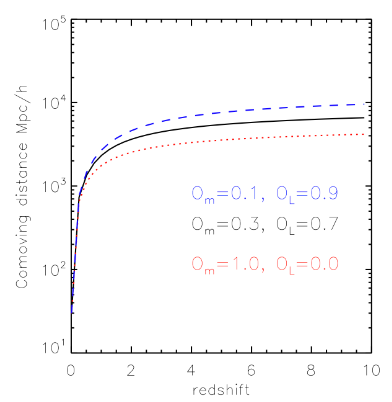
\includegraphics[width=0.309\textwidth]{GA8/共动距离-红移关系}
    \caption{共动距离-红移关系}
\end{figure}


\subsubsection{宇宙的年龄}
由$\dot{a}=\frac{da}{dt}$, 即$dt=\frac{da}{\dot{a}}$得
\begin{align*}
    t(z)=\int_0^{a(z)}\frac{da}{\dot{a}}=\frac{1}{H_0}\int_z^\infty\frac{dz}{(1+z)E(z)}
\end{align*}
回溯时间(lookback time),即从红移z到目前$z=0$的年龄
\begin{align*}
    t_b(z)=t_0-t=\frac{1}{H_0}\int_0^z\frac{dz}{(1+z)E(z)}
\end{align*}
这里$\frac{1}{H_0}$是哈勃时标, $\sim 9.78\times 10^9$/hyr

\begin{figure}[!htb]
    \centering
    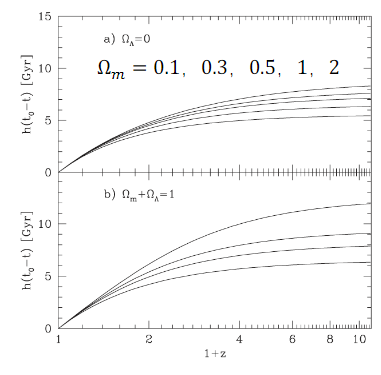
\includegraphics[width=0.309\textwidth]{GA8/宇宙的年龄}
    \caption{宇宙的年龄}
    \label{宇宙的年龄}
\end{figure}
图\ref{宇宙的年龄} 给出回溯时间对宇宙学参数的依赖关系. 

\subsubsection{视界 (Horizon)}

\begin{figure}[!htb]
    \centering
    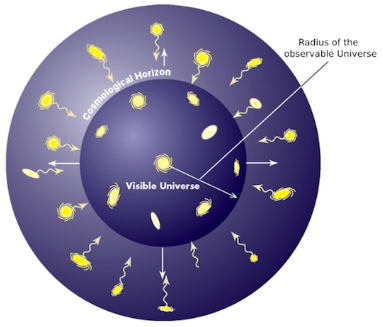
\includegraphics[width=0.24\textwidth]{GA8/视界 (Horizon)}
    \caption{视界 (Horizon)}
\end{figure}

在宇宙某一时刻, 视界, $D_h(t)$ , 定义为从宇宙诞生之时, 到观测者所在时间, 光子能传播的最大固有距离, 由\ref{E1}, 与推导\ref{E10}类似, 但$t=0$对应于红移$z=\infty$
\begin{align}
    \chi(r_e)=\frac{c}{H_0 a_0}\int_z^\infty\frac{dz}{E(z)} \label{E11}
\end{align}
因此
\begin{align*}
    D_h(z)=a\chi=\frac{c}{H_0 (1+z)}\int_z^\infty\frac{dz}{E(z)}
\end{align*}
由于E(z)随z增
加而衰减很快, 实际计算中, $z$可以取一个较大的值, 如10000, 结果就相对精确. 

图\ref{宇宙视界与红移} 为平坦宇宙下, 不同宇宙学参数下, 宇宙视界与红移的关系. 
\begin{itemize}\small
    \item 视界随着时间而增加
    \item 宇宙学常数越大, 宇宙膨胀越快, 界越大. 
\end{itemize}

\begin{figure}[!htb]
    \centering
    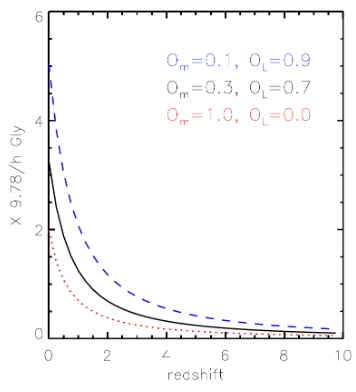
\includegraphics[width=0.309\textwidth]{GA8/宇宙视界与红移}
    \caption{宇宙视界与红移}
    \label{宇宙视界与红移}
\end{figure}

\subsubsection{光度距离与红移的关系}
由$d_L=a_0(1+z)r_e$代入\ref{E10}得
\begin{align*}
    d_L=(1+z)\frac{c}{H_0}\int_0^z\frac{dz}{E(z)}
\end{align*}
距离模数$m-M=5\log(\frac{d_L}{10pc})$可得其与红移的关系. 利用SN-Ia, 可以独立测量其红移$z$(谱线移动)和距离模数(SN-Ia的绝对星系和视星等都可以测量). 

\begin{figure}[!htb]
    \centering
    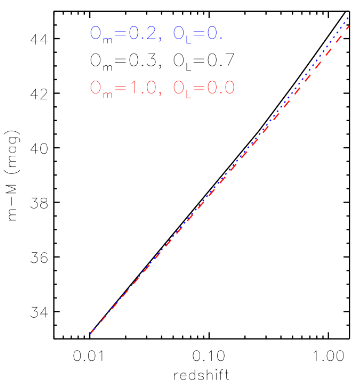
\includegraphics[width=0.309\textwidth]{GA8/光度距离与红移的关系}
    \caption{光度距离与红移的关系}
\end{figure}
\begin{itemize}\small
    \item 注意, 光度距离对宇宙学参数的依赖较弱, 因此需要高精度的测量才能确定暗能量参数. 
    \item 高红移数据对宇宙学参数差别大, 但目前$z>1$的数据较少. 
\end{itemize}

\subsection{宇宙膨胀因子随时间的变化}
考虑几种简单情况下, $a$随时间变化
\begin{enumerate}
    \item 辐射为主时期, 宇宙早期, 辐射主导$(\sim a^{-4})$, \ref{E7}简化为
    \begin{align*}
        \left( \frac{\dot{a}}{a} \right)^2=\frac{8\pi G}{3}\rho_{r,0}\left( \frac{a_0}{a} \right)^4
    \end{align*}
    可以积分得到
    \begin{align}
        \left( \frac{\dot{a}}{a} \right)^2=\left( \frac{32\pi G \rho_{r,0}}{3} \right)^{\frac{1}{4}}t^{\frac{1}{2}}\label{E12}
    \end{align}
    \item 物质为主时期, 且假设$\Lambda=0$, \ref{E7}为
    \begin{align*}
        \left( \frac{\dot{a}}{a} \right)^2=H_0^2\left[ \Omega_{m, 0}\left( \frac{a_0}{a} \right) ^3 - \frac{K c^2}{H_0^2a_0^2}\left( \frac{a_0}{a} \right)^2\right]
    \end{align*}
    \begin{enumerate}
        \item For $K=0$
        \begin{align*}
            \frac{a}{a_0}=\left( \frac{3}{2}H_0 t \right)^{\frac{2}{3}}
        \end{align*}
        这就是著名的Einstein-de Sitter (EdS)宇宙. 
        \item For $K=-1$
        \begin{align*}
            \frac{a}{a_0}&=\frac{1}{2}\frac{\Omega_{m, 0}}{1-\Omega_{m, 0}}(\cosh \vartheta -1)\\
            H_0 t&=\frac{\Omega_{m, 0}}{(1-\Omega_{m, 0})^{\frac{3}{2}}}(\sinh \vartheta-\vartheta)
        \end{align*}
        $\vartheta\in (0, \infty)$
        \item For $K=1$
        \begin{align*}
            \frac{a}{a_0}&=\frac{1}{2}\frac{\Omega_{m, 0}}{\Omega_{m, 0}-1}(1-\cos \vartheta)\\
            H_0 t&=\frac{\Omega_{m, 0}}{(\Omega_{m, 0}-1)^{\frac{3}{2}}}( \vartheta-\sin\vartheta)
        \end{align*}
        $\vartheta\in (0, 2\pi)$, $a$存在一个最大值在 $t_{max}$时刻, $\frac{a_{max}}{a_0}=\frac{\Omega_{m, 0}}{\Omega_{m, 0}-1}$, 之后宇宙塌缩到$a=0$. 
    \end{enumerate}
    \item 物质为主平坦宇宙, 即$\Omega_{m, 0}+\Omega_{\Lambda, 0}=1$, \ref{E7}化简为
    \begin{align*}
        \left( \frac{\dot{a}}{a} \right)^2=H_0^2\left[ \Omega_{m,0}\left( \frac{a_0}{a} \right) +\Omega_{\Lambda, 0}\right]
    \end{align*}
    当随着宇宙膨胀, 物质项可以忽略时
    \begin{align*}
        \frac{a}{a_0}=\exp\left[ \Omega_\Lambda^{\frac{1}{2}}H_0(t-t_0) \right]
    \end{align*}
    这就是著名的 de Sitter 宇宙, 即宇宙指数膨胀. 
    \subitem For $0<\Omega_{m, 0}<1$, (目前观测支持的模型), 膨胀因子的严格解为
    \begin{align}
        \frac{a}{a_0}=\left( \frac{\Omega_{m, 0}}{\Omega_{\Lambda, 0}} \right)^{\frac{1}{3}}\left[ \sinh\left( \frac{3}{2}\Omega_{\Lambda, 0}^{\frac{1}{2}}H_0 t \right) \right]^{\frac{2}{3}}\label{E13}
    \end{align}
    根据该表达式, 早期$a\propto t^{\frac{2}{3}}$, 即 Einstein-de Sitter Unvierse. 晚期$a\propto\exp\left[ \Omega_\Lambda^{\frac{1}{2}}H_0(t-t_0) \right]$, 即 de Sitter 宇宙. 
    \item 其他, 对于包含宇宙学常数, 且$K\ne 0$的情况, $a$随时间演化更加复杂, 这里不再讨论可以参考<Galaxy Formation and Evolution>, by Mo et al. book
\end{enumerate}

\subsection{宇宙的创生(普朗克时期)}
目前大爆炸理论认为宇宙来自于$\sim$138亿前的大爆炸. 大爆炸之前没有时间, 没有空间, 只有真空. 充满了量子涨落的``沸腾的真空''. 根据量子力学的测不准原理, 时间涨落与能量涨落满足
\begin{align*}
    \Delta t\Delta E\ge \frac{h}{4\pi}
\end{align*}
$h$为普朗克常数. 在宇宙早期, 辐射主导, 由\ref{E12}知$\rho_{r, 0}=\sigma T^4$, 此外辐射温度满足$\frac{T}{T_0}=\frac{a_0}{a}$, 可以得到宇宙的温度与时间的关系为
\begin{align*}
    T=\left( \frac{3c^2}{32\pi G \sigma} \right)^{\frac{1}{4}}t^{-\frac{1}{2}}
\end{align*}
可以看到宇宙温度与目前时刻的温度$T_0$没有依赖关系. 宇宙的总能量$E\cong \sigma T^4 a^3\sim KT$,因此由测不准关系
\begin{align*}
    tE\approx tKT=K \left( \frac{3c^2}{32\pi G \sigma} \right)^{\frac{1}{4}}t^{\frac{1}{2}}=\frac{h}{4\pi}
\end{align*}
代入相关系数, 可以得到$p_{pl}\approx 6\times 10^{-44}$s, 其对应的能量$E_{pl}\approx 1.2\times 10^{19}GeV$, 对应温度$10^{32}$K. $t_{pl}, E_{pl}$分别称为普朗克时间, 普朗克能量. 光子在普朗克时间内传播的距离为$10^{-35}$m, 该尺度称为普朗克长度. 与普朗克能量对应的质量$m_{pl}=\frac{E_{pl}}{c^2}=2.2\times 10^{-5}$g. 

普朗克时间, 尺度的意义: 它们代表了经典连续时空中能测量的最小时间和空间间隔. 在更小的尺度上, 时间和空间不连续了, 即量子化了. 

宇宙大爆炸可以看着是一次$t\rightarrow 0, E\rightarrow \infty$的一次真空能释放. 从质能角度看, 相当于``无中生有'', 创造了物质. 

宇宙各处都在普朗克时间内发生了爆炸, 因此总能量远远大于普朗克能量. 

\subsection{宇宙的暴胀}
在上世纪80年代, 人们发现标准宇宙大爆炸模型碰到了严重困难, 即如何解释宇宙的空间平直性和视界问题, 于是提出了宇宙暴胀模型. 

\subsubsection{平直性问题}
在没有宇宙学常数的模型下, Friedmann方程写为
\begin{align*}
    1=\frac{8\pi G}{3H^2}\rho-\frac{K}{H^2 a^2}\ (k=0, -1, 1)
\end{align*}
定义$\Omega=\frac{\rho}{\rho_c}=\frac{8\pi G \rho }{3H^2}$, 可得
\begin{align*}
    1-\frac{1}{\Omega}=\frac{3K}{8\pi G \rho a^2}
\end{align*}
在辐射为主时期, $\rho \propto a^{-4}$, 物质为主时期, $\rho\propto a^{-3}$, 因此有
\begin{align*}
    \left| 1-\frac{1}{\Omega} \right|\propto |K| \times \begin{array}{ll}
        a^2 &\text{辐射为主} \\
        a   &\text{物质为主} \\
    \end{array}
\end{align*}
因此, 无论$k=0/1$, 在宇宙早期, 等式右边趋近于0,  即$\Omega=1$, 宇宙表现为平直空间. 但是当$a$很大时,  $\Omega$与1有明显偏离. 

从宇宙爆炸至今, 宇宙从普朗克时间($10^{-44}$s), 从辐射为主($t=10^4$yr$=10^{11}$s)到物质为主的今天($10^17$s), 宇宙尺度因子的变化为, 
\begin{align*}
    \frac{a_0}{a_{pl}}=\frac{a_{eq}}{a_{pl}}\frac{a_0}{a_{eq}}=\left( \frac{10^{11}}{10^{-43}} \right)^{\frac{1}{2}}\times \left( \frac{10^{17}}{10^{11}} \right)^{\frac{2}{3}}=10^{31}
\end{align*}
同时从爆炸至今$\left| 1-\frac{1}{\Omega} \right|$的变化为
\begin{align*}
    \frac{\left| 1-\frac{1}{\Omega} \right|_{t_0}}{\left| 1-\frac{1}{\Omega} \right|_{t_{pl}}}=\left( \frac{a_{eq}}{a_{pl}} \right)^2\frac{a_{t_0}}{a_{eq}}\approx 10^{58}
\end{align*}
从几率角度看, 很难理解. 为什么早期宇宙的密度和哈勃常数$(\rho,H)$应该是两个相互独立的随机量, 但是它们给出的组合量$\Omega$却非常精确的等于1, 与1的偏差只是在小数点后面58位. 即宇宙诞生之初, 其曲率应该$K=0$. 

\subsubsection{视界问题}

从宇宙爆炸到微波背景形成的时刻$t_R$, 光线传播的共动距离
\begin{align*}
    \chi=\int_0^{t_R}\frac{dt}{a(t)}
\end{align*}
在$t_R$以前, 宇宙基本为辐射主导, 即$a(t)\propto t^{\frac{1}{2}}$, 因此
\begin{align*}
    \chi=\frac{1}{a_R}2t_R
\end{align*}
此外, 光子从$t_R$时刻到现在走过的共动距离, 在物质主导时
\begin{align*}
    a\sim t^{2/3},\ d=\int_{t_R}^{t_0}\frac{dt}{a(t)}=\frac{3t_0}{a_0}
\end{align*}
因此,  该视界在空间的张角
\begin{align*}
    \theta=\frac{r}{d}=\frac{2}{3}\left( \frac{1}{1+z_R} \right)^{1/2}
\end{align*}
微波背景辐射对应于$z_R\sim 1000$, 得到$\theta\sim 1.8^{\circ}$. 即有物理联系的区域不超过$1.8^{\circ}$. 

\begin{figure}[!htb]
    \centering
    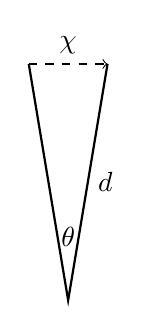
\begin{tikzpicture}
        \draw [thick] (-0.5, 0)--(0, -3)--(0.5, 0) node [midway, right] {$d$};
        \node at(0, -2.2) {$\theta$};

        \draw [dashed, ->] (-0.5, 0)--(0.5, 0) node [midway, above] {$\chi$};
    \end{tikzpicture}
\end{figure}

观测发现, CMB的辐射在全天的温度基本均匀, 因此有物理因果关系, 需要再次证明宇宙需要经历一个暴胀阶段. 

\subsubsection{宇宙暴胀理论-Inflation}
暴胀模型有多种.  GUT (大统一理论)认为, 暴胀发生在真空发生相变的时刻. 假设宇宙处于真空状态, 但宇宙学常数不为0, 即 $\rho=0$, $\Lambda>0$.由Freedmann方程 \ref{E4} 可得
\begin{align*}
    \ddot{a}-\frac{\Lambda c^2}{3}a=0
\end{align*}
可以求解得到
\begin{align*}
    a=a_{if}e^{\sqrt{\frac{\Lambda c^2}{3}}t}
\end{align*}
$a_{if}$ 为宇宙暴胀开始时刻宇宙的大小. 可以看到宇宙暴胀时, 宇宙尺度因子按指数增长. 

大统一理论认为暴胀发生在宇宙温度为$T_c\sim 10^{15}$Gev时刻, 该时刻之前, 宇宙为辐射主导. $a\sim T^{-1}\propto t^{1/2}$, 
由$1ev \cong 1.16*10^4 k$T, 结合宇宙在普朗克时间的温度为$10^{32}$K, 可以知道暴胀发生在$t\approx 10^{-35}$s, 当时真空能密度$\rho_{\Lambda}=\frac{\Lambda c^3}{8\pi G}\sim T_c^4$, 因此有
\begin{align*}
    H=\sqrt{\frac{\Lambda c^2}{3}}=10^{35}/s
\end{align*}
按照GUT理论, 暴涨过程从$t\approx 10^{-35}$s开始, 持续到$t\approx 10^{-33}$s结束. 宇宙在此过程中膨胀了 $e^{10^{35}(10^{-33}-10^{-35})}=e^{100}=10^{43}$倍.  

将尺度因子 $a\sim e^{\sqrt{\frac{\Lambda c^2}{3}}t}$ 代入Freedmann \ref{E6}, 且设密度为$\rho =0$, 可得$K=0$. 宇宙尺度因子的暴胀可以看成是宇宙曲率因子的急剧膨胀, 如一个二维球面, 不管其之前的曲率半径为多少, 急剧暴胀后曲率半径变成无穷大, 球面可以看成平面. 因此暴胀解决了``宇宙平直性''问题. 

\begin{figure}[!htb]
    \centering
    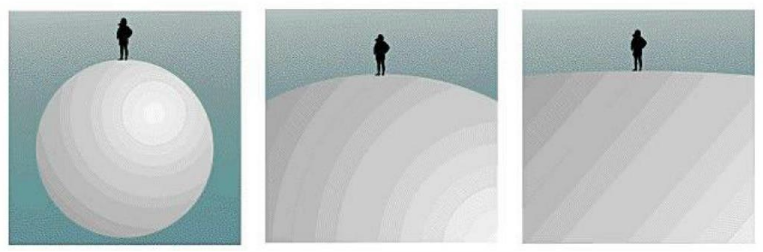
\includegraphics[width=0.48\textwidth]{GA8/暴胀让宇宙变得平坦}
    \caption{暴胀让宇宙变得平坦}
\end{figure}

\begin{figure}[!htb]
    \centering
    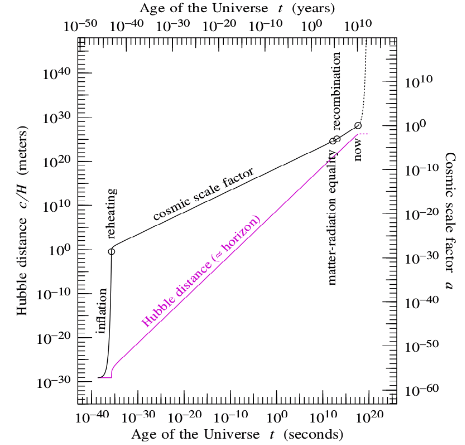
\includegraphics[width=0.309\textwidth]{GA8/视界问题}
    \caption{视界问题, 左轴: 视界尺度. 右轴: 尺度因子}
\end{figure}


视界问题: 
\begin{itemize}\small
    \item 视界正比于宇宙年龄, 从当前时间反推到普朗克时间, 视界从$10^{10}$光年缩小到$10^{-43}$光秒, 两者相比为$10^{60}$倍. 
    \item 空间区域大小正比于宇宙尺度因子$a(t)$, 如果没有暴胀, 从现在($10^{10}$光年)到普朗克时间, 观测的空间区域将缩小$10^{31}$倍. 
    \item 视界的大小会远小于空间尺度, 产生视界疑难. 
\end{itemize}
加入暴涨, 宇宙空间区域的大大缩小, 因此空间尺度远远小于视界尺度. 就使得我们今天看到的全部宇宙, 完全可以在宇宙暴胀前处在同一个有因果联系的区域, 解决了``视界''问题. 

\subsection{宇宙演化史}
目前关于早期宇宙的演化还知之甚少, 有许多模型. 一般认为宇宙经历如下阶段: 
\begin{enumerate}\small
    \item 普朗克时期: 从大爆炸开始到$10^{-43}$秒, 最小的时间单位, 期间物理过程基本不了解
    \item 大一统时期: 从$10^{-43}$秒到$10^{-36}$秒, 重力与其他作用力(电弱力)分离. X,Y玻色子产生
    \item 电弱时期: $10^{-36}$到$10^{-12}$秒, 强核力从电弱力分量, 各种基本粒子(W,Z,X,Y玻色子及希格斯玻色子产生), 宇宙暴涨产生并结束, 宇宙由夸克-胶子等离子体, 光子组成. 
    \item 夸克时期: $10^{-12}$到$10^{-6}$秒, 四种基本作用力完全分开. 
    \item 强子时期: $10^{-6}$到1秒, 宇宙温度$\sim10^9$K, 夸克形成强子, 包括质子, 中子. 
    \item 轻子时期: 1秒$\sim$10秒, 强子和反强子相互湮灭. 
    \item 光子时期: $\sim 10$秒, 轻子和反轻子湮灭, 电子和正电子湮灭, 剩下少数电子
    \item 元素核合成: 3分钟$\sim$20分钟, 质子和中子形成原子核, 最终形成氢, 氦. 
    \item 辐射主导:  10秒$\sim$60,000年, 光子与原子核, 电子组成等离子体, 并与其有相互作用
    \item 复合时期: $\sim$380, 000年, 宇宙温度$\sim$3000K, 自由电子消失, 光子开始自由穿梭
    \item 黑暗时期: 380, 000年$\sim$1-2亿年, 宇宙中没有恒星, 只有光子. 暗物质开始聚集成团
    \item 再电离时期: 2$\sim$7亿年, 第一代恒星, 星系形成, 宇宙再次变得透明, 完成再电离
    \item 大量结构形成: 7亿年-138亿年, 银河系形成, 太阳系形成
\end{enumerate}
$10^{-6}$s之前都是猜的, 380000年时形成微波背景辐射. 

% \subsection{宇宙热历史(Thermal history)}
% 30-31 跳过了

% 以下+1了
\subsection{宇宙早期物理过程---轻元素合成}
宇宙原初核合成.

当宇宙温度下降到$\sim 10^{10}$K时, 夸克-胶子等离子体形成稳定的强子后, 电子与质子通过如下弱作用过程而相互转化:
\begin{align*}
    n+e^+&\rightleftharpoons p+\bar{v}_e\\
    n+v_e&\rightleftharpoons p+e^-\\
    n&\rightleftharpoons p+e^-+\bar{v}_e
\end{align*}
这里$v_e,\ \bar{v}_e$表示电子型中微子及其反粒子. 由于中子与质子的静止质量之间差异为$Q=(m_n-m_p)c^2=1.3$Mev, 因此热平衡时, 其密度并不相等, 两者之比由玻尔兹曼公式给出, 
\begin{align*}
    \frac{n_n}{n_p}=\left( \frac{m_n}{m_p} \right)^{3/2}\exp\left( -\frac{Q}{KT} \right) \approx \exp\left( -\frac{Q}{KT} \right)
\end{align*}
即中子数略少于质子数. 当温度低于0.87Mev时(宇宙年龄$\sim$2秒), 上面的弱相互作用反应率小于宇宙膨胀速率, 中子和质子之间停止相互转化, 其数密度``冻结'', 定义中子数与全部核子数之比为
\begin{align*}
    X_n(0)=\frac{n_n}{n_n+n_p}=\left[ 1+\exp\left( \frac{Q}{KT} \right) \right]^{-1}\approx 0.17
\end{align*}
这一比值可以维持到宇宙年龄$t_n\sim 20$秒, 宇宙温度$\sim 3.3\times 10^9$K. 此外, 自由中子寿命为$\tau_n \approx 886$秒, 会衰变为质子, $n\rightarrow p+e^-+\bar{v}_e$, 因此$X_n(0)$ 随时间演化为
\begin{align*}
    X_n(t)=X_n(0)\exp\left( -\frac{t-t_n}{\tau_n} \right)\approx X_n(0)e^{-t/\tau_n}
\end{align*}

当宇宙温度进一步降低到$\sim 10^9$K ($t\sim 270$s)时, 中子和质子开始形成氘( ${}^2H$ or $D$, $D$的结合能为2.2MeV,只有当温度$<10^9$K, $D$才能形成), 
\begin{align*}
    p+n&\rightarrow B+\gamma\\
    D+p&\rightarrow {}^3He+\gamma\\
    D+D&\rightarrow {}^3He+n\\
    D+D&\rightarrow {}^3H+p\\
    {}^3He+n&\rightarrow {}^3H+p
\end{align*}
最终通过
\begin{align*}
    {}^3He+D&\rightarrow {}^3He+p\\
    {}^3H+D&\rightarrow {}^4He+n
\end{align*}
形成稳定的氦 . 一旦$D$形成, 上述反应很快进行, 将所有中子都结合到氦核, 因此$D$生成时( $t_D\sim 270$s)的中子丰度$X_n=X(0)\exp(-t_D/ \tau_n )=0.125$,此时氦的丰度为(质量比)
\begin{align*}
    Y=\frac{2n_n}{n_n+n_p}\approx 0.25
\end{align*}
伽莫夫等人于1948年得到了上述结果. 剩下的氢元素质量占比$\sim 75\%$. 事实上, $He$生成以后还会产生少量的锂元素. 上述核合成过程大约持续到宇宙爆炸后3分钟. 

\begin{figure}[!htb]
    \centering
    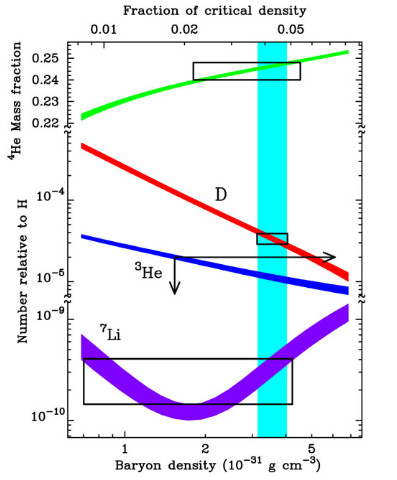
\includegraphics[width=0.309\textwidth]{GA8/轻元素核合成}
    \caption{轻元素核合成}
    \label{轻元素核合成}
\end{figure}


上述标准模型预言的轻元素丰度与宇宙中总重子密度密切相关. 图\ref{轻元素核合成} 表明, 目前观测的原初氦元素丰度与重子密度关系与理论非常符合. 表明大爆炸宇宙学模型的正确性. 宇宙中比锂更重的元素都来自恒星内部核反应, 并通过星风和超新星爆炸, 将它们转移星际空间. 

\subsection{宇宙热力史---复合时期}

\begin{enumerate}
    \item 宇宙微波背景辐射(CMB)
    \item $2.7\pm 10^{-5}$K
    \item $t_{age}=3.8\times 10^5$yr
    \subitem ($T>3000$K, H电离)
\end{enumerate}

{\small 轻元素合成以后, 宇宙继续为辐射主导, 一直到$\sim 40000$年宇宙变为物质主导, 但是此时宇宙温度足够高, 物质(重子)还是处于电离状态, 一直到宇宙$\sim380000$年, 温度下降到4000K时, 自由电子和原子核开始结合为原子, 光子不再与电子/质子发生散射, 从而在宇宙中自由穿行, 形成宇宙背景辐射. 光子穿行到今天, 其温度下降到2.7K,辐射峰值在微波波段($\sim 1$mm), 因此称为宇宙微波背景辐射(Cosmic Microwave Background). }

\begin{figure}[!htb]
    \centering
    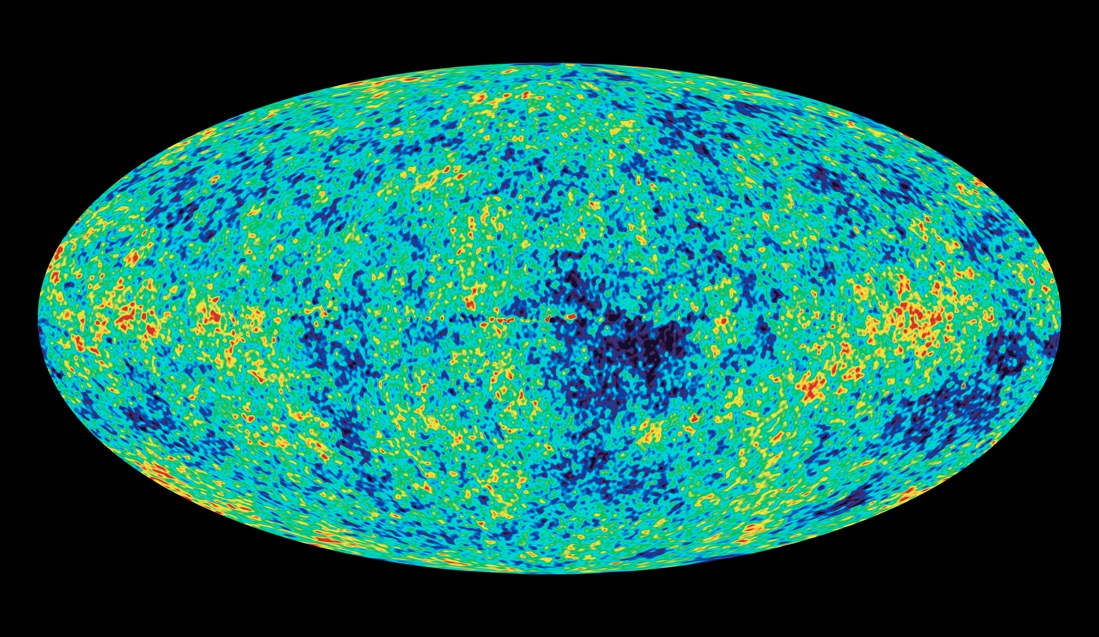
\includegraphics[width=0.309\textwidth]{pic/GA8/CMB.jpg}
    \caption{宇宙微波背景辐射}
\end{figure}

\subsubsection{复合时期温度计算}
对于氢原子, 其电离能$E=13.6$eV, 对应温度$\sim 1.6*10^5 $K. 而温度4000K 时, 对应的光子平均能量为0.34 eV, 但宇宙中光子数目与重子数目比非常大, 只要光子中存在一部分能量高于$E$的``高能尾巴'', 则原子将保持电离. 

在温度$T$时, 宇宙背景辐射为黑体, 其能谱分布为普朗克公式, 
\begin{align*}
    f(\nu, T)d \nu=\frac{8 \pi h \nu^3}{3}\frac{1}{e^{h\nu /kT}-1}d\nu
\end{align*}
总光子密度可由在某个频率范围$(\nu, d\nu)$内的光子密度$dN(\nu, T)=f(\nu, T)d\nu /h\nu$积分而得. 
\begin{align*}
    N(T)&=\frac{8\pi k^3 T^3}{h^3 c^3}\int_0^\infty \frac{x^2}{e^x -1}dx \\
    &=19.23\pi\left( \frac{kT}{hc} \right)^3 \approx 420(1+z)^3/\text{cm}^3
\end{align*}
$x=\frac{h\nu}{kT}$

宇宙重子密度
\begin{align*}
    n_B=&\Omega_B\rho_c(1+z)^3/m_p\\
    &\approx 1.12\times 10^{-5}(1+z)^3\Omega_B h^2/\text{cm}^3
\end{align*}
宇宙中光子与重子数密度之比为
\begin{align*}
    \frac{n_r}{n_B}\approx 3.8\times 10^7 (\Omega_B h^2)^{-1}
\end{align*}
取$\Omega_B h^2\sim 0.02$, 比值可高达$10^9$. 

单位体积内, 能量$h\nu \ge E$的光子数与总光子数之比为
\begin{align*}
    \beta=\frac{n(h\nu \ge E)}{N}\approx \frac{1}{N}\int_{E/h}^\infty \frac{8\pi \nu^3}{c^3}\frac{d \nu}{e^{h\nu/kT}-1}
\end{align*}
令$y=\frac{E}{kT}$, 可得$\beta(y)=\frac{1}{0.24\pi^2}e^{-y}(y^2+2y+2)$, 取$\beta(y)=1o^{-9}$, 可得$y=E/kT\approx 26.5$. 

如果取$E$为氢原子的基态能量13.6eV, 可得$T\sim 6000$K. 此时占光子总数$1/10^9$的光子(与重子数相当)的高能光子可以让所有氢原子电离. 更为详细的计算表明即使$T\sim 4500$K, 也有足够的光子将氢原子先从基态跃迁到第一激发态, 其余光子再使他们从激发态电离. 

在辐射与重子脱藕过程中, 定义电离率
\begin{align*}
    x=\frac{n_e}{n}
\end{align*}
$n_e$为自由电子的数密度, $n$为氢原子加上自由电子的数密度, 在热平衡条件下, 氢原子的电离平衡由Saha公式给出, 
\begin{align*}
    \frac{n_e n_p}{n_H n}=\frac{x^2}{1-x}=\frac{(2\pi m_e kT)^{3/2}}{nh^3}e^{-B/kT}
\end{align*}
这里$n_p$为氢粒子的数密度$(n_p=n_e)$, $n_H=n-n_p$为中性氢原子的数密度, $B$=13.6eV为基态氢原子的电离能. 取$T=2.73(1+z)$K, $n=1.12\times 10^{-5}(1+z)^3\Omega_B h^2 /\text{cm}^3$, 可以得到
\begin{align*}
    \log\left( \frac{x^2}{1-x} \right)=21.0-\log\left[ \Omega_B h^2(1+z)^{3/2} \right]-2.5*\frac{10^4}{1+z}
\end{align*}
可以看到在z<1100时, 电离率很快衰减. 因此宇宙中绝大部分氢原子保持中性, 光子可以自由穿梭. 

\begin{figure}[!htb]
    \centering
    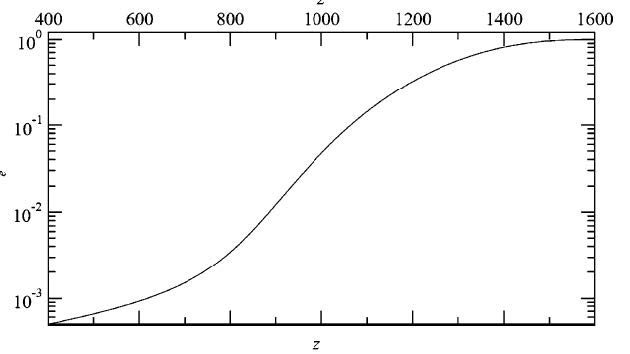
\includegraphics[width=0.42\textwidth]{GA8/x随红移的变化}
    \caption{x随红移的变化}
\end{figure}

\subsubsection{CMB最大的扰动尺度}
\begin{figure}[!htb]
    \centering
    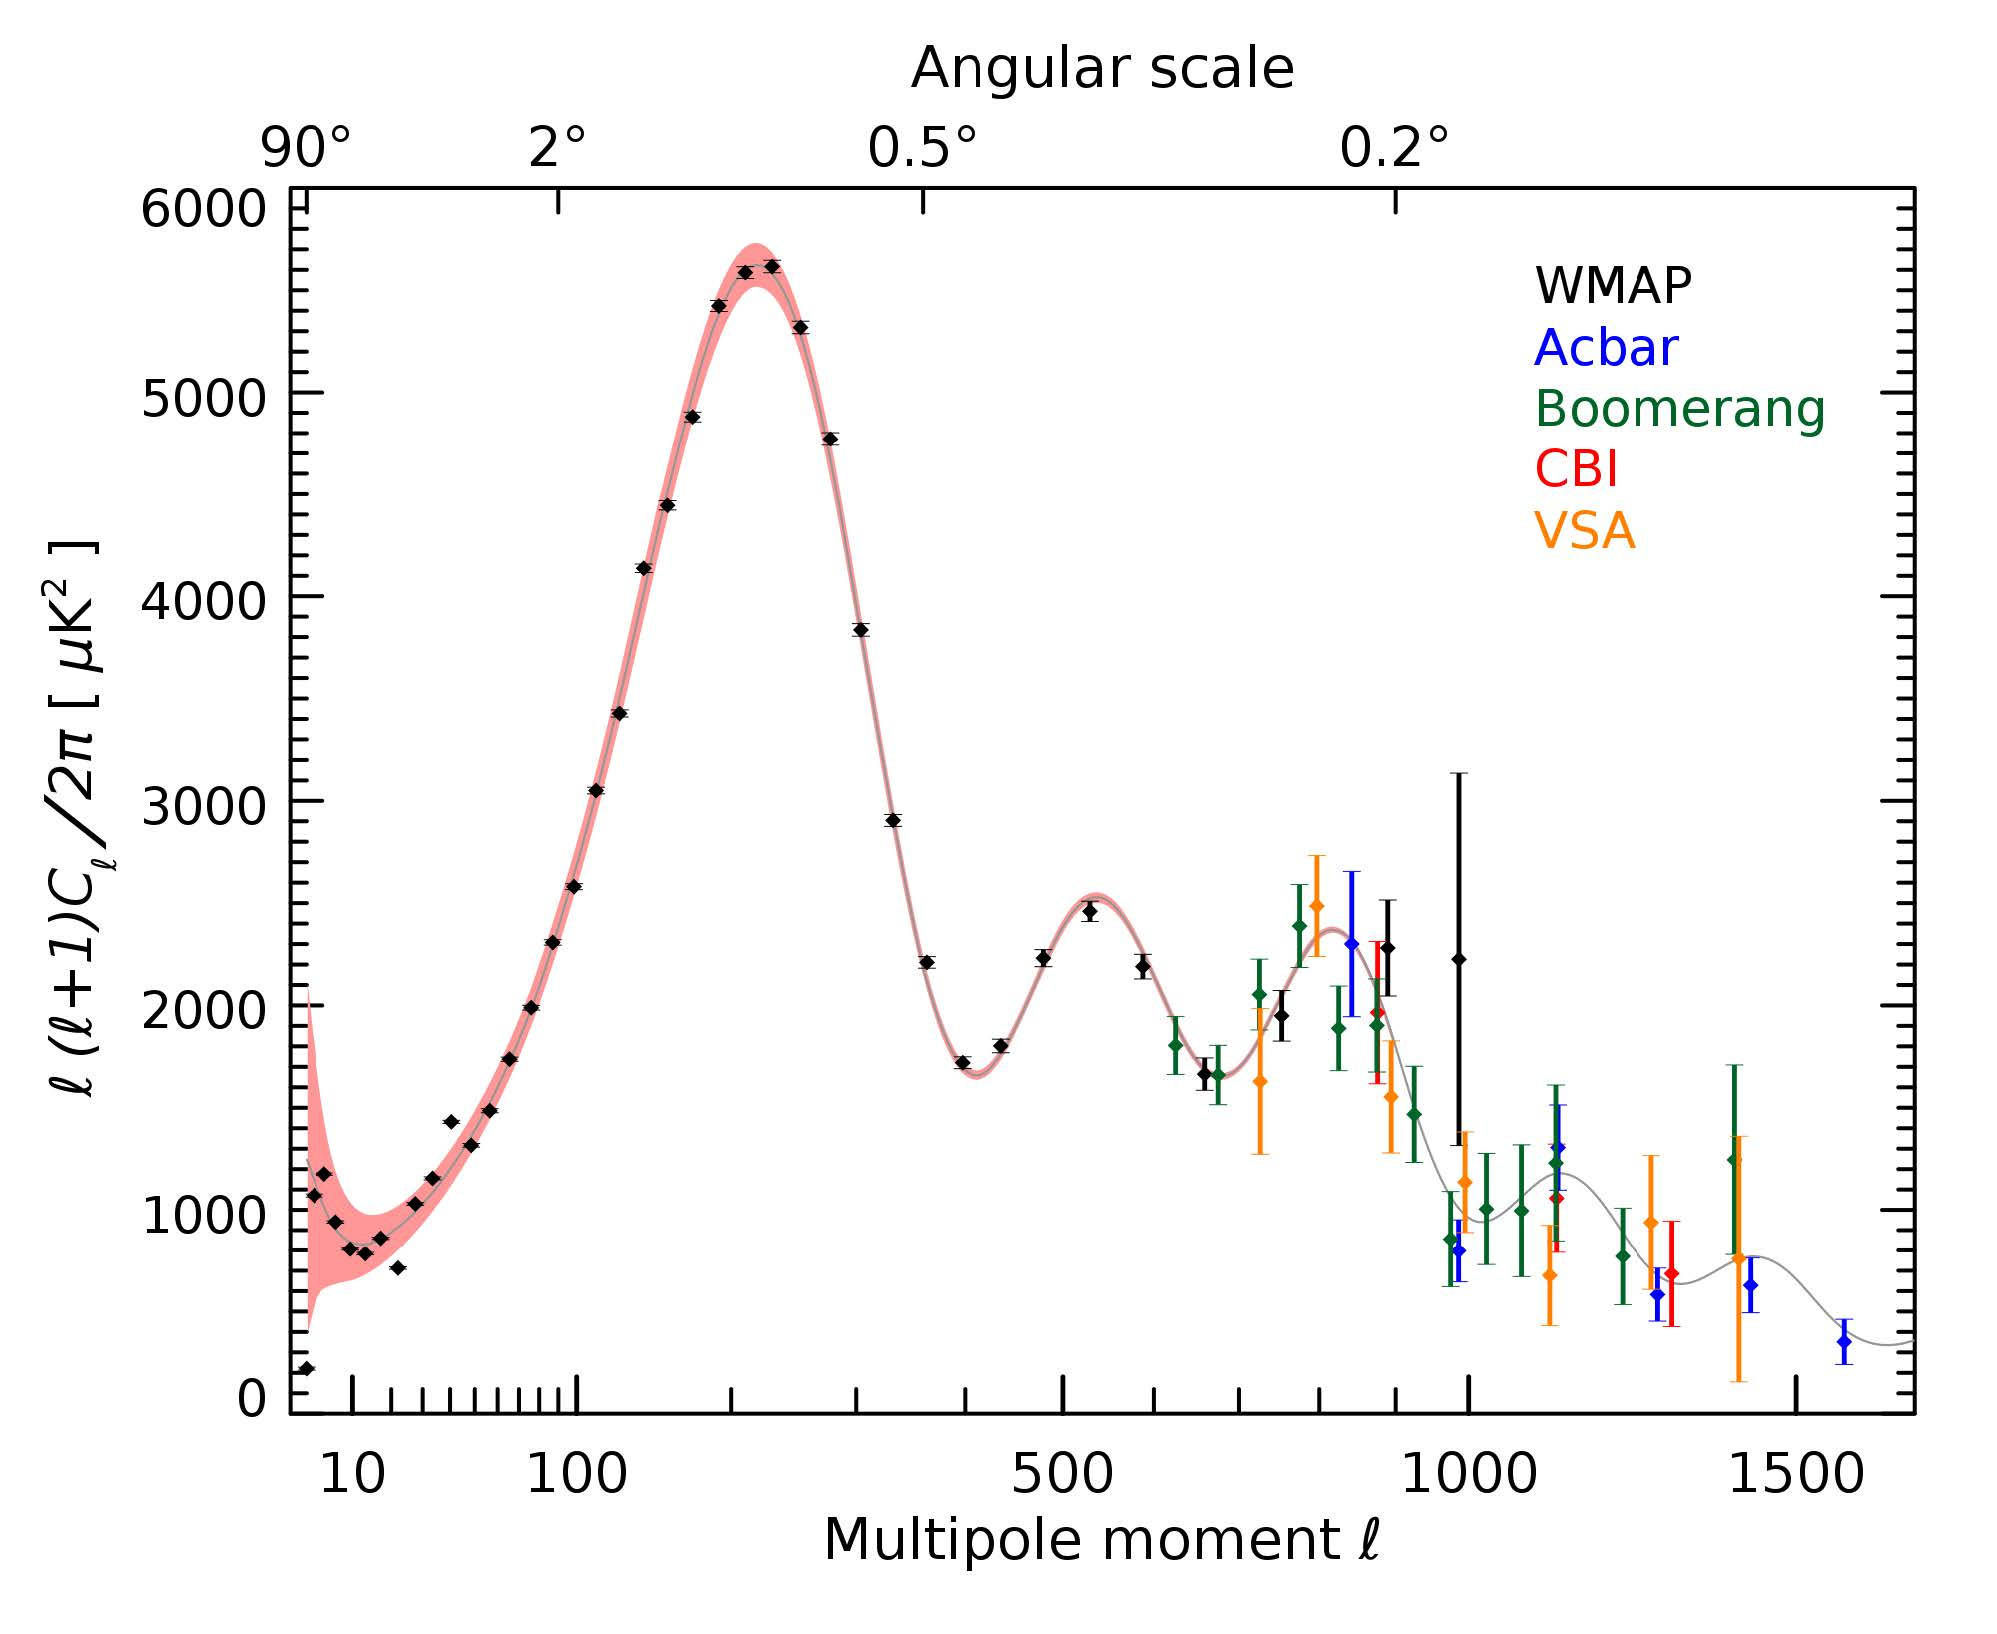
\includegraphics[width=0.42\textwidth]{GA8/扰动角度}
    \caption{扰动角度}
    \label{扰动角度}
\end{figure}

由日常经验可知, 对于某种震动引起的波, 其在$t$时间范围内传播的距离为
\begin{align*}
    d=c_s t
\end{align*}
$c_s$为波的声速. 在复合开始前, 光子和电子通过康普顿散射发生很强的相互作用, 可以视为单一流体, 其声速$c_s\sim 0.45 c$. 

从大爆炸到再复合时期, 该声波传播的共动距离为
\begin{align*}
    r=\int_0^t\frac{c_s dt}{a(t)}
\end{align*}
而微波背景辐射距离我们的共动距离$D(z=1100)$可以很容易计算, 因此该扰动的最大角度
\begin{align*}
    \theta=\frac{r}{D}
\end{align*}
通过计算, 可以发现$\theta\sim 0.8^{\circ}$ ,对应$l=250$,对应图 \ref{扰动角度} 的第一个峰. 

注: $z=1100$时刻,宇宙视界$\sim2* 0.8^{\circ} $(光速传播)


